\section{Project Status}

\subsection{Code}
We have created the necessary Jupyter notebooks and python scripts to generate distributions of interest and their perturbations. This includes code to save those distributions to HDF5 files. We developed a framework in C++ for loading those HDF5 distributions and their perturbations and generating the corresponding octrees, adding the perturbations to the particles and then rebalancing the octree. This allows us to observe the effects of the initial construction as well as across varying magnitudes of perturbations. This will be important in developing our final report as it will be important to show how varying magnitudes of perturbations generate correlate to the rebalancing time for trees. This relates to Cornerstone's flagship feature which is allowing rebalancing rather than rebuilding. 

\subsection{Machines}
Currently we have used \href{https://www.cloudlab.us/}{CloudLab} to gain access to GPUs allowing us to get preliminary results on a node with 4 V100s; however, access to this is difficult to attain on a regular basis. 

\subsection{Algorithms}


\subsection{Results}
A general test to develop a sense of Cornerstone's internal bottlenecks is done on a single GPU comparing a case with 100 million using either Hilbert or Morton keys. The test loop contains the code to compute the SFC, do a radix sort, reorder the corresponding particle properties, and update the leaves and then internal tree state; these are the steps needed to compute the octree and have it be in a usable state. Immediately we see that the sorting and reordering of particle properties is very dominant in this regime.

\begin{figure}[h!]
    \centering
    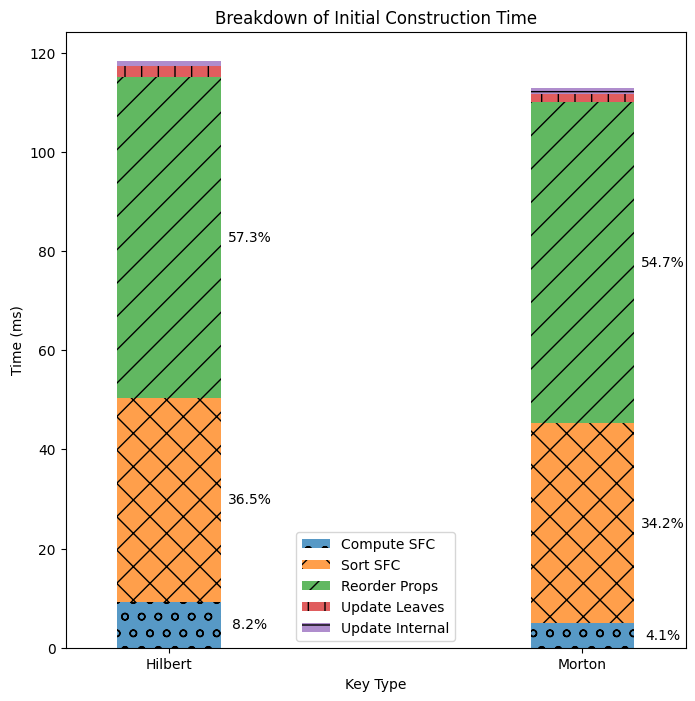
\includegraphics[width=0.45\textwidth]{assets/init_100m.png}
    \caption{Comparison of operations in a broader tree update on a single GPU.}
    \label{fig:keys_100m}
\end{figure}
